\subsection{Optimal settings 
for CMA-ES \label{optimalsettingscma}}

When finding the optimal settings for CMA-ES we have a larger set of parameters we can adjust compared
to the Cross-entropy method. Again, as the same with the Cross-entropy method, we can adjust the population/parent size and
games per agent. Furthermore we can adjust the initial step-size, lower bound and recombination type.\\
The following sections will go into detail how these parameters affect the performance of CMA-ES
algorithm. In the last section we will perform experiments to determine the optimal settings.

%In previous sections we focused on tuning Cross Entropy for the Tetris 
%problem. Whereas we deliberately chose not to tune CMA due to its implementation 
%into the Shark library \citep{shark08}. However, experiments with the "out of 
%the box" CMA from Shark, with default settings vs the tuned Cross Entropy
%resulted in CMA reaching convergence very fast but not achieving the same point
%limit as Cross Entropy.\\

\subsubsection{Recombination type}
CMA-ES has a unique formula for calculating the updated mean,
called the 'Recombination type'. Where the recombination type
determines how much influence each of the offspring vectors has on the next
generation. Built into the CMA-ES algorithm is three methods of recombination. 
\begin{itemize}
\item Equal
\item Linear
\item Superlinear
\end{itemize}
By default, CMA-ES uses Superlinear recombination. However, Tetris is a problem
with multiple local optimums and heavy noise in its search space. This means, though a vector may be the best in its generation, it could be a nearby local optimum. Therefore, Superlinear recombination may not be the optimal recombination type for the Tetris problem.\\

The recombination types are covered in section \ref{CMAtheory} on 
page \pageref{eq:recomType}.


\subsubsection{Population and selection size}
By adjusting the population size to that similar of the Cross-entropy method, we are able
to get a fair comparison between the two algorithms, given each generation will
contain the same number of agents. By setting the population and parent size
to the same values, we in effect test if the covariance matrix and the step-size
control has a impact on the algorithm performance compared to the Cross-entropy method
which does not have the features.\\
Table \ref{CMAPopulationSelectionConfigTest} displays the values that we are going
to test for the population and selection size.


\begin{table}[H]
\centering
\begin{tabular}{r r}
Population size, $\populationSize$ & Parent size, $\offspringNumber$\\
\hline
$13$ & $1$\\
$13$ & $3$\\
$13$ & $6$\\
$22$ & $2$\\
$22$ & $5$\\
$22$ & $11$\\
$50$ & $5$\\
$50$ & $12$\\
$50$ & $25$\\
$100$ & $10$\\
$100$ & $25$\\
$100$ & $50$
\end{tabular}
\caption{CMA-ES configuration for population and parent size \label{CMAPopulationSelectionConfigTest}}
\end{table}

The experiments includes different population $N \in \{13,22,50,100\}$ and offspring sizes of either
10\%, 25\% and 50\%. We use 10\% because of the Cross-entropy method recommended selection size, while
we use 25\% because of CMA-ES' standard selection size for the Equal recombination type. 
Furthermore we use 50\% because of CMA-ES' standard selection size for the Linear and Superlinear 
recombination type.

\subsubsection{Games per agent \label{CMAGamesPerAgentSection}}
As with the Cross-entropy method we can also adjust the number of games each agent plays per generation.
However, because of the recombination type for CMA-ES, one game pr. agent may  be insufficient to assess the
performance of an agent. The Linear and Superlinear recombination types will value the better agents higher.
Therefore, it may occur that some better-on-average agent encounter an unlucky game, achieving a lower score than
it's actual potential allows. \\
Thus, evaluating each agent multiple times and using the average score for recombination may allow for a more accurate assessment.\\

The experiments includes different games per agent of $\{1,3,5,7,10\}$. We have chosen the same 
values as with the Cross-entropy method to get comparable results (see section \ref{GamesPerAgentCESection}).

\subsubsection{Initial step-size \label{sec:CMAInitialStepSize}}
Initially, the covariance matrix of CMA-ES in generation $\generation = 0$
is the identity matrix. The initial step-size, $\sigma_0$, will hence in 
the first iteration scale the area in which the CMA-ES algorithm searches.
As from section \ref{normalSamples}, it's known that the scale of the 
solutions has no impact on the scores. Hence, it's assumed that the initial 
step-size should not have any major impact on the results.

\begin{figure}[H]
\centering
\begin{tabular}{r | r r r r r}
$\sigma_0$ & mean & Q1 & Q2 & Q3\\
\hline
0.1 & 50769.3 & 21301.1 & 54588.7 & 73972.4\\
0.2 & 42290.6 & 32180.2 & 42290.6 & 49337.4\\
0.5 & 53893.7 & 14211.1 & 66773.0 & 85816.7\\
0.8 & 37557.7 & 1422.8  & 15450.8 & 93719.4\\
1.0 & 49537.9 & 31369.8 & 49537.4 & 58454.6
\end{tabular}
\caption{Results of CMA-ES with adjusted initial step-size \label{CMAInitialSigmaConfigTest}}
\end{figure}
The full graphs of the results from this experiment can be seen in 
appendix \ref{appendixCMAInitialSigma}.\\
For the initial experiments using CMA-ES, 
the only adjusted parameter is the initial 
step-size $\sigma_0$. The configurations of step-sizes were 
$\sigma_0 \in \{0.1, 0.2, 0.5, 0.8, 1.0\}$. As the table shows,
the final mean score does not seem to change with the initial step-size.
Furthermore, the adjustment of the step-sizes does not appear to 
have a drastic impact on the mean scores. However, based on both mean score and
quantiles, the best configuration seems to be $\sigma_0 = 0.5$. This is 
is also referred to as a typical initial setting in \citep{boumaza2009}.
Therefore, the conclusion remains that the initial step-size is not critical 
for the experiment.\\

To tell if the step-size is actually a significant parameter to adjust, results from 
the two best performing configurations are compared using the Mann-Whitney-Wilcoxon test\footnote{\url{https://stat.ethz.ch/R-manual/R-patched/library/stats/html/wilcox.test.html}}.
The Mann-Whitney-Wilcoxon test has the appealing property that it does not require any parameters
besides the actual data to test, and it does not require the assumption that data originates 
from a Gaussian distribution. The test accepts data from two populations, that may or may not 
be drawn from the same underlying distribution and will test against the null hypothesis, 
namely that the two populations have identical distribution. If the test concludes a 
confidence less then $5\%$ ($p < 0.05$), we cannot firmly reject the null hypothesis, 
and cannot conclude any significant difference in the population. From the experiments
with the initial sigma setting, the immediate choice of $\sigma_0$ would be 0.5.
The Wilcoxon test is applied to the data from the runs with $\sigma_0 \in \{0.5, 1\}$
using R\footnote{\url{https://cran.r-project.org/}}. The data supplied
to the wilcoxon test consists of the the mean scores from the last generation.
This test gives $p=0.5619$, which means that we cannot reject that the two 
populations differ, and the initial sigma is considered not to play a significant 
for the CMA-ES applied to Tetris.

\subsubsection{Lower bound}

As with the Cross-entropy method, to avoid early convergence
at a too low local optimum, a 
certain lower threshold for the variance should be applied when 
sampling vectors for solutions. In the Cross-entropy method, a constant 
noise term $z^{(\generation)} = 4$ is added to the variance for each component
of the sampled vectors. When the $i$'th component in the Cross-entropy method is
sampled as follows
\begin{align*}
\individual_i &\sim \mathcal{N}\left(m, \sigma^{2}\right)\\
              &\sim \sigma \mathcal{N}\left(m, 1\right)
\end{align*}
Then $\sigma^{2} \geq 4$. To gain the same effect for the CMA-ES, a lower bound 
is applied to the step-size. Such a bound is implemented in the Shark library
as the following, where the value of the lower bound is $l$
\begin{align*}
\sigma  \lambda_n \geq l
\end{align*}
Here $\lambda_n$ is the lowest eigenvalue in the covariance matrix. 
When the vectors are sampled, the samples are scaled by the matrix $D$
containing the eignvalues of the covariance matrix. 
Hence, if $\sigma \lambda_n \geq l$, then the smallest scaling
that takes place is at least $l$. As the vectors can be written 
as
\begin{align*}
\individual &\sim \mean + \sigma B 
\underbrace{D \mathcal{N}\left(0, I \right)}_{\mathcal{N}\left(0, D^2 \right)}
\end{align*}
Where $D \mathcal{N}\left(0, I \right)$ corresponds to 
$\mathcal{N}\left(0, D^2 \right)$ which, since $D$ is a diagonal
matrix, is just the same type of sampling as with the Cross-entropy method. 
The matrix $B$ will only rotate the the sampled vectors, and finally,
$\sigma$ will perform an isotropic scaling. 
To roughly resemble the constant noise configuration of the Cross-entropy method,
when sampling vectors, the lowest variance may not drop below 4. 
This is achieved by setting a lower bound $l=2$. If this applies,
the sampling can be written as
\begin{align*}
\individual &\sim \mean +  B \mathcal{N}\left(0, \sigma^2 D^2 \right)
\end{align*}
Where, with $l=2$, the lowest entry in the diagonal matrix $\sigma^2 D^2$
is $4$.\\
\\
To see if this setting makes sense, the CMA-ES was run with lower bounds as 
$l \in \{0.5, 2.0, 4.0\}$ with the results shown in figure \ref{CMALowerBoundConfigTest}.

\begin{figure}[H]
\centering
\begin{tabular}{r | r r r r r}
$l$ & mean & Q1 & Q2 & Q3\\
\hline
0.5 & 42800.7 & 6780.8  & 36863.0 & 74722.5\\
2.0 & 80733.4 & 62357.4 & 84349.0 & 108007.5\\
4.0 & 61497.2 & 55621.7 & 64940.1 & 81991.6\\
\end{tabular}
\caption{Results of CMA-ES lower bounds \label{CMALowerBoundConfigTest}}
\end{figure}
The raw graphs for this experiment is present in appendix \ref{appendixCMALowerBound}.\\
Evidently, the setting of a lower bound $l=2.0$ appears as the preferable choice, and this 
setting adopted across all further experiments.


\subsubsection{Experiment for finding the optimal settings \label{OptimalSettingsCMA}}
In this in section we are going to conduct a wide variety of experiments to determine
the best settings for CMA-ES. More specifically we are going to find the best combination for
population size, parent size and games per agent.\\
Table \ref{SuperCMAExperiment} depict the different experiments we are
going to carry out.

\begin{table}[H]
\centering
\begin{tabular}{c c l c}
Population Size & Parent size & Recombination Type & Games per Agent\\
\hline
$13$ & $1$ & EQUAL/LINEAR/SUPERLINEAR & 1/3/5/7/10\\
$13$ & $3$ & EQUAL & 1/3/5/7/10\\
$13$ & $6$ & LINEAR/SUPERLINEAR & 1/3/5/7/10\\
$22$ & $2$ & EQUAL/LINEAR/SUPERLINEAR & 1/3/5/7/10\\
$22$ & $5$ & EQUAL & 1/3/5/7/10\\
$22$ & $11$ & LINEAR/SUPERLINEAR & 1/3/5/7/10\\
$50$ & $5$ & EQUAL/LINEAR/SUPERLINEAR & 1/3/5/7/10\\
$50$ & $12$ & EQUAL & 1/3/5/7/10\\
$50$ & $25$ & LINEAR/SUPERLINEAR & 1/3/5/7/10\\
$100$ & $10$ & EQUAL/LINEAR/SUPERLINEAR & 1/3/5/7/10\\
$100$ & $25$ & EQUAL & 1/3/5/7/10\\
$100$ & $50$ & LINEAR/SUPERLINEAR & 1/3/5/7/10
\end{tabular}
\caption{Full experiments overview for finding the optimal settings for CMA-ES\label{SuperCMAExperiment}}
\end{table}

The choice behind using the above population sizes is to use the same population sizes as
when we tuned the Cross-entropy method (see section \ref{optimalsettingsce}).\\
In regards to the parent size, they have been determined depending on the recombination type.
We use all three different recombination types for the 10\% parent sizes to make these experiments
correspond to the Cross-entropy method settings (see section \ref{optimalsettingsce}). However, Shark CMA-ES
has predetermined parent sizes for each recombination types, 25\% for Equal and 50\% for both
Linear and Superlinear \citep{shark08}. For this reason we also conduct experiments for each population
size to represent these Shark CMA-ES preferred settings.
Furthermore we also test different number of games per agent as for the reason presented in section \ref{CMAGamesPerAgentSection}.\\\\
These experiments will be conducted using Hard Tetris (see section \ref{HardTetris}), in order
to lower the computation time.\\

\textbf{Results}\\
The total number of configuration experiments is 120, with 30 individual experiments each,
resulting in a total of 3.600 individual experiment runs. These results are all included in 
appendix \ref{appendixCMAPopulationParent}.\\
Below in table \ref{CMABestConfigTable} and figure \ref{CMABestConfigPlot}, the four best
best resulting configurations are depicted. We chose these by first selecting the best 
configuration of each Population-Parent size with each recombination type. This resulted in six
configurations for each Population-Parent size, which we then compared to determine the best
configuration for each Population-Parent size, regardless of recombination type. Which is depicted in table \ref{CMABestConfigTable} and figure \ref{CMABestConfigPlot}.

\begin{table}[H]
\centering
\small
\begin{tabular}{c c l c r r r r}
Population & Parent & Recombination & Games per Agent & Mean & Q1 & Q2 & Q3\\
\hline
$13$ & $6$  & SUPERLINEAR & 10 & $2472.293$ & $2194.049$ & $2430.780$ & $2709.040$\\
$22$ & $11$ & SUPERLINEAR & 10 & $2849.220$ & $2500.231$ & $2835.450$ & $3143.121$\\
$50$ & $25$ & SUPERLINEAR & 5  & $3211.658$ & $2889.689$ & $3305.485$ & $3694.480$\\
$100$ & $50$ & LINEAR     & 7  & $3322.076$ & $3160.098$ & $3289.370$ & $3537.850$
\end{tabular}
\caption{Best performing configurations of all population sizes \label{CMABestConfigTable}}
\end{table}

\begin{figure}[H]
\centering
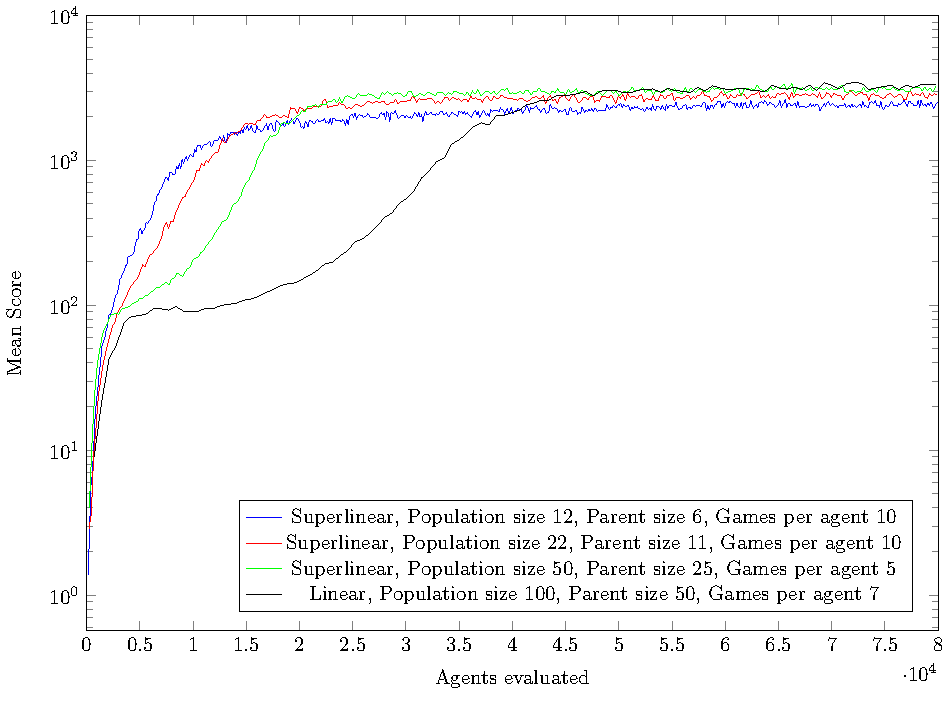
\includegraphics[scale=0.8]{data/cma_population_offspring/bestofall_population/PlotFile.pdf}
\caption{Best performing configurations of all population sizes \label{CMABestConfigPlot}}
\end{figure}

From table \ref{CMABestConfigTable} and figure \ref{CMABestConfigPlot}, we can see that
Linear recombination type, with population size 100, parent size 50 and 7 games per agent
(black) yields a better score compared to Superlinear with population size 50, parent size 25 and 5 games per agent (green).
However, green has a much faster convergence than black and almost reaches the same score.\\

\textbf{Analysis and discussion}\\
Because the green converges almost twice as fast as black, but reaches practically the same
score, we opt to use the Superlinear with population size 50, parent size 25 and 5 games per agent for the comparison experiments.\\
Therefore, we will be using this configuration for the tuned comparison experiments.








